%%%%%%%%%%%%%%%%%%%%%%%%%%%%%%%%%%%%%%%%%
% Short Sectioned Assignment
% LaTeX Template
% Version 1.0 (5/5/12)
%
% This template has been downloaded from:
% http://www.LaTeXTemplates.com
%
% Original author:
% Frits Wenneker (http://www.howtotex.com)
%
% License:
% CC BY-NC-SA 3.0 (http://creativecommons.org/licenses/by-nc-sa/3.0/)
%
%%%%%%%%%%%%%%%%%%%%%%%%%%%%%%%%%%%%%%%%%

%----------------------------------------------------------------------------------------
%	PACKAGES AND OTHER DOCUMENT CONFIGURATIONS
%----------------------------------------------------------------------------------------

\documentclass[paper=a4, fontsize=11pt]{scrartcl} % A4 paper and 11pt font size

\usepackage[T1]{fontenc} % Use 8-bit encoding that has 256 glyphs
\usepackage{fourier} % Use the Adobe Utopia font for the document - comment this line to return to the LaTeX default
\usepackage[english]{babel} % English language/hyphenation
\usepackage{amsmath,amsfonts,amsthm} % Math packages
\usepackage{amssymb}

\usepackage[T1]{fontenc}
\usepackage[scaled]{beramono}
\usepackage{listings}

\usepackage{algpseudocode}
\usepackage{algorithm}

\usepackage{graphicx}
\DeclareGraphicsExtensions{.png}
\graphicspath{{./imgs/}}

\usepackage{subcaption}

\usepackage{sectsty} % Allows customizing section commands
\allsectionsfont{\normalfont\scshape} % Make all sections centered, the default font and small caps
%\renewcommand{\thesection}{}

% Shove the number into the margin, and places a dot after it.
\makeatletter
\def\@seccntformat#1{\protect\makebox[0pt][r]{\csname
the#1\endcsname.\quad}}
\makeatother

\newtheorem{theorem}{Theorem}[section]
\newtheorem{corollary}{Corollary}[theorem]
\newtheorem{lemma}[theorem]{Lemma}
% For external Lemmas and Theorems
\newtheorem*{theorem*}{Theorem}
\newtheorem*{lemma*}{Lemma}

\usepackage{fancyhdr} % Custom headers and footers
\pagestyle{fancyplain} % Makes all pages in the document conform to the custom headers and footers
\fancyhead{} % No page header - if you want one, create it in the same way as the footers below
\fancyfoot[L]{} % Empty left footer
\fancyfoot[C]{} % Empty center footer
\fancyfoot[R]{\thepage} % Page numbering for right footer
\renewcommand{\headrulewidth}{0pt} % Remove header underlines
\renewcommand{\footrulewidth}{0pt} % Remove footer underlines
\setlength{\headheight}{13.6pt} % Customize the height of the header


\numberwithin{equation}{section} % Number equations within sections (i.e. 1.1, 1.2, 2.1, 2.2 instead of 1, 2, 3, 4)
\numberwithin{figure}{section} % Number figures within sections (i.e. 1.1, 1.2, 2.1, 2.2 instead of 1, 2, 3, 4)
\numberwithin{table}{section} % Number tables within sections (i.e. 1.1, 1.2, 2.1, 2.2 instead of 1, 2, 3, 4)

\setlength\parindent{0pt} % Removes all indentation from paragraphs - comment this line for an assignment with lots of text

\newcommand{\set}[1]{\{#1\}}
\newcommand{\setoneto}[1]{\set{1,2,\ldots,#1}}

\DeclareMathOperator{\OO}{O}
\DeclareMathOperator{\fl}{float}
\DeclareMathOperator{\cut}{\delta}
% \DeclareMathOperator(\ZZ}{\ensuremath{\mathbb{Z}}}
% \DeclareMathOperator(\RR}{\ensuremath{\mathbb{R}}}
%\DeclareMathOperator{\lg}{lg}
\newcommand{\ceil}[1]{\left\lceil#1\right\rceil}
\newcommand{\abs}[1]{\left\lvert#1\right\rvert}
\newcommand{\floor}[1]{\left\lfloor#1\right\rfloor}
\newcommand{\trans}[1]{#1^\intercal}
\newcommand{\opt}[1]{\mathbf{#1}}
%----------------------------------------------------------------------------------------
%	TITLE SECTION
%----------------------------------------------------------------------------------------

\newcommand{\horrule}[1]{\rule{\linewidth}{#1}} % Create horizontal rule command with 1 argument of height

\title{\
    \normalfont\normalsize
    \textsc{University of Waterloo} \\ [25pt] % Your university, school and/or department name(s)
    \horrule{0.5pt} \\[0.4cm] % Thin top horizontal rule
    \huge CS 759 Report:\\
    Killing Time \\
    \horrule{2pt} \\[0.5cm] % Thick bottom horizontal rule
}

\author{Theo Belaire \\ 20415730 \\ Bryan Coutts \\ 20428420} % Your name

\date{\normalsize\today} % Today's date or a custom date

\begin{document}

\maketitle % Print the title


Some terminology, I use the term \textit{included} point to refer to points
that are to be included inside the blob, and \textit{excluded} points to refer
to points that must be on the exterior of the blob.

Unless specified, polygon can mean non-convex polygon. \\

Our algorithm works as follows:
\begin{enumerate}
\item Take the convex hull of the included points.
\item Fix the convex hull, so that no excluded points are in its interior.
\item Compute the radii for each point.
\item Induct nearby points to the polygon. 
\item Remove ``crossover'' points.
\item Draw blob around the vertices of the polygon.
\end{enumerate}


\section{Generation of the Convex Hull}
Our code uses the giftwrap algorithm to generate the convex hull.
This runs in $\OO(i^2)$ time, where $i$ is the number of points included in the
set. \\

It works by picking the leftmost point, and calculating the angle that is
formed with each other point in the set, and picking the point that forms
the angle closest to a straight line with the previous point. \\

% TODO nice diagram of in progress giftwrap?
At the conclusion of this step, we have a list of included points in clockwise
order, which forms our polygon $P$. Currently it is convex.

\section{Point Exclusion}
In this step, we will fix $P$, so that no excluded point is in its interior. We
will do so by removing triangles from $P$; this will cause it to no longer be
convex. \\

To test if an excluded point is within $P$, we use the Jordan Curve Theorem. One
of its consequences is that if we trace a ray from the point in any direction,
it will cross an edge of $P$ an even number of times if and only if the point is
outside $P$.  This is computationally simple to check. \\

For each excluded point $p$ in the interior of $P$, we find the edge closest to
$p$. We consider only the edges whose endpoints $p$ is between.  We then insert
$p$ into our list of polygon vertices, between the endpoints of this edge. This
removes the triangle formed by the edge and $p$ from $P$.


\section{Calculating Radii}
The \textit{radius} of a point determines how large a circle is used when
drawing the blob around it. If all the radii were very small, the blob would
appear the same as the polygon.  However, the radii cannot be too large,
otherwise the circles draw around included and excluded points will intersect
with each other. Hence, the radius of an included point is bounded by its
distance to an excluded point, and vice-versa. Moreover, there are situations in
which the radius of an included point must be bounded by its proximity to
another included point, as illustrated in ~\ref{fig:neck}.

\begin{figure}[h]
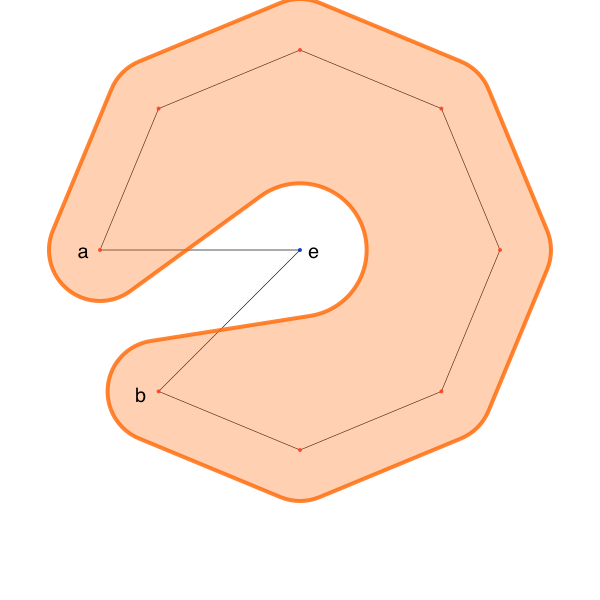
\includegraphics[width=0.5\textwidth]{torus_bitten}
\centering
\caption{``If the radii of $a,b$ are too large, the blob will self-overlap''}
\label{fig:neck}
\end{figure}

For included points $a,b$, $a$ must bound the radius of $b$ if and only if the
line segment from $a$ to $b$ is contained entirely within $P$. Similarly, for
excluded points $a,b$, $a$ must bound the radius of $b$ if and only if the line
segment from $a$ to $b$ is disjoint from $P$. We check this condition by
checking if any edges of the polytope intersect with the line segment from $a$
to $b$. \\

Given this notion of which points bound each others' radii, we choose the radius
of a point to be $1/3$ of its distance to the nearest bounding point. This
ratio must be at most $1/2$ to avoid overlap. The smaller the ratio is, the
thinner and blockier our blob will be. $1/3$ allows for a curvy blob, while
avoiding some pinching effects observed with higher ratios.

\section{Inducting nearby points}
Once we have all the radii, we almost know the final shape of the blob. However,
there may be excluded points near the edge of the polygon, whose circles (or
even the points themselves) may intersect the blob, as seen in
~\ref{fig:whyrefine}. There may also be included points near the border, whose
circles would intersect the exterior of the blob.  We add all such points to the
polygon.

\begin{figure}[h]
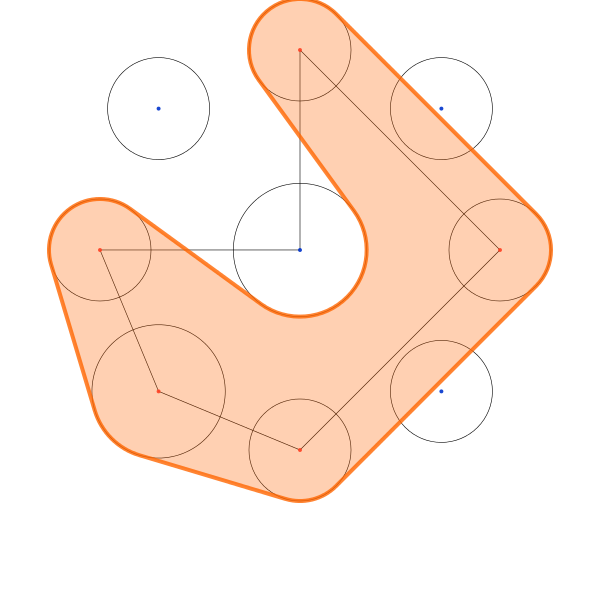
\includegraphics[width=0.3\textwidth]{whyrefine}
\centering
\caption{``The circle of the bottom-right point is cut by the blob''}
\label{fig:whyrefine}
\end{figure}

We iterate over all points $p$ that are not vertices of $P$. Then, for each edge
$e = (a,b)$ of $P$, we check if the line from the edge of the circle of $a$ to
the edge of the circle of $b$ intersects the circle of $p$. If it does, we add
$p$ to $P$, between $a$ and $b$ (effectively adding the trangle with vertices
$a,b,p$ to $P$). \\

\begin{figure}
        \centering
        \begin{subfigure}[b]{0.5\textwidth}
                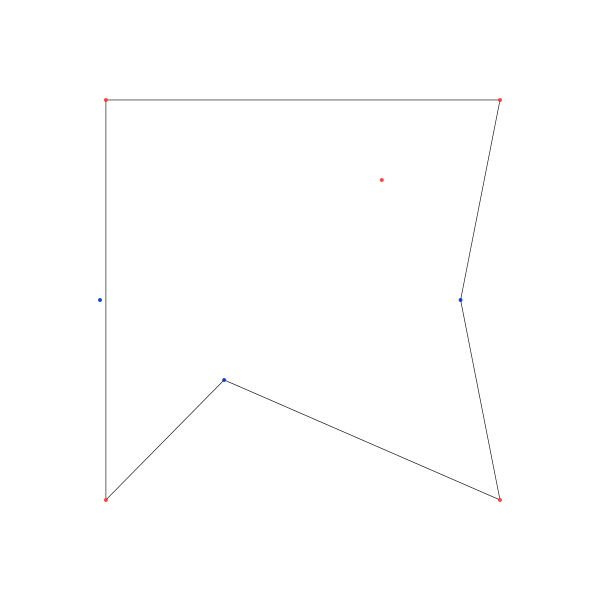
\includegraphics[width=\textwidth]{before_caving}
                \caption{Before}
                \label{fig:before}
        \end{subfigure}%
        ~ %add desired spacing between images, e. g. ~, \quad, \qquad, \hfill etc.
          %(or a blank line to force the subfigure onto a new line)
        \begin{subfigure}[b]{0.5\textwidth}
                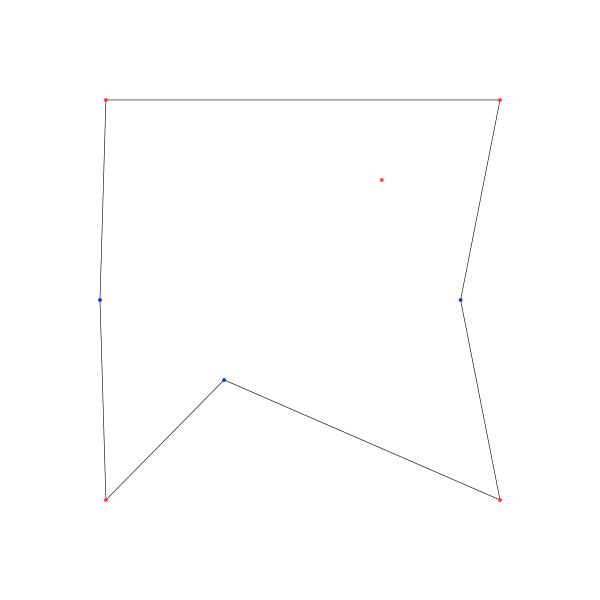
\includegraphics[width=\textwidth]{after_caving}
                \caption{After}
                \label{fig:after}
        \end{subfigure}
        \caption{Before and After caving}\label{fig:caving}
\end{figure}

\section{Uncrossing}

\section{Arc computation}
Once we have a final boundary, and radii, we can draw the blob.

For each edge $uv$, we consider a pair of circles centered at
$u$ and $v$, with the radii $r_u$ and $r_v$.

Consider as if we were to take a piece of string and wrap it around
the outside of these circles.
It would have three segments,
first when it was in contact with the first circle,
then it would leave and travel along a line tangent to both circles,
then it would arrive at the second circle
and travel along it before leaving somewhere on the other side.




% \begin{figure}[h]
% \includegraphics[width=\textwidth]{7/folder}
% \caption{''It's number 7''}
% \end{figure}
\end{document}
